\documentclass[a4paper,11pt]{article}

% --- Packages ---
\usepackage[utf8]{inputenc}
\usepackage{geometry}
\usepackage{graphicx}
\usepackage{tikz}
\usepackage{hyperref}
\usepackage{titlesec}
\usepackage{parskip}
\usepackage{float}
\usepackage{xcolor}
\usepackage{enumitem}
\usepackage{booktabs}
\usepackage{fancyhdr}

% --- TikZ Libraries ---
\usetikzlibrary{shapes, arrows, positioning, fit, backgrounds, shadows, calc}

% --- Setup ---
\geometry{margin=1in}
\hypersetup{
    colorlinks=true,
    linkcolor=blue,
    urlcolor=blue
}
\pagestyle{fancy}
\fancyhf{}
\rhead{Hedera RWA Architecture}
\lhead{Tokenised NCD Factory}
\cfoot{\thepage}

% --- Title ---
\title{\textbf{Automated Issuance Architecture for\\Tokenised Negotiable Certificates of Deposit (NCDs)}}
\author{Technical Design Document \\ Target Network: Hedera (HSCS \& HTS)}
\date{\today}

% --- TikZ Styles ---
\tikzstyle{block} = [rectangle, draw, fill=blue!10, text width=6em, text centered, rounded corners, minimum height=3em, drop shadow]
\tikzstyle{entity} = [rectangle, draw, fill=green!10, text width=5em, text centered, minimum height=2.5em, drop shadow]
\tikzstyle{line} = [draw, -latex']
\tikzstyle{cloud} = [draw, ellipse, fill=red!10, node distance=3cm, minimum height=2em]
\tikzstyle{container} = [draw, rectangle, dashed, inner sep=1em, fill=gray!5]

\begin{document}

\maketitle

\begin{abstract}
This document outlines a "Factory-based" architecture for deploying Tokenised Negotiable Certificates of Deposit (NCDs) on the Hedera network. The design leverages the Hedera Token Service (HTS) for asset safety and the Smart Contract Service (HSCS) for logic enforcement. We propose a segregated architecture where an \textbf{ERC-4626 Vault} manages custody and maturity enforcement, while separate \textbf{Entry/Exit Adapters} manage the pricing logic required for Australian-style Discount Securities. This approach maximizes composability, auditability, and risk isolation.
\end{abstract}

\tableofcontents
\newpage

% =============================================================================
% SECTION 1: INTRODUCTION
% =============================================================================
\section{Introduction}

The digitization of Real World Assets (RWA) is shifting from manual, bespoke deployments to automated, API-driven factories. This architecture addresses the specific requirements of the Australian Money Market, where NCDs are treated as \textbf{Discount Securities} (purchased below par, redeemed at par).

\subsection{The Problem}
Current DeFi standards (like ERC-4626) assume a "Deposit Asset X $\to$ Get Asset X" workflow. However, a Discount NCD requires a "Pay Currency Y $\to$ Get Debt Token X" workflow. Furthermore, institutional issuance requires strict isolation of risk per deal.

\subsection{The Solution: The "Deal Factory"}
We introduce a design where a single JSON Request for Quote (RFQ) triggers the atomic deployment of a dedicated environment for that specific deal. This isolates the asset, the maturity logic, and the liquidity pool from all other deals on the platform.

% =============================================================================
% SECTION 2: HEDERA ADVANTAGE
% =============================================================================
\section{Why Hedera?}

While this architecture could exist on Ethereum, Hedera provides three distinct advantages for institutional RWA:

\begin{enumerate}
    \item \textbf{HTS (Native Assets):}
    On Ethereum, a token is a smart contract ($ERC20.sol$). If the contract has a bug, the asset is lost. On Hedera, the token is a native ledger entity. The smart contract \textit{wraps} the token but does not \textit{contain} it. This significantly reduces "Smart Contract Risk."

    \item \textbf{Token Association (Anti-Spam/Compliance):}
    Hedera requires accounts (and contracts) to explicitly "Associate" with a token before receiving it. This prevents "Dusting attacks" and ensures that the Vault contract explicitly opts-in to manage the NCD asset.

    \item \textbf{Finality \& Cost:}
    Fixed fees (\$0.05 USD for associations/transfers) allow for precise business modeling, unlike gas-auction markets.
\end{enumerate}

% =============================================================================
% SECTION 3: ARCHITECTURAL DESIGN
% =============================================================================
\section{Architectural Design}

The system follows a \textbf{Segregated Responsibility} pattern. We separate the \textit{Storage of Value} from the \textit{Transaction Logic}.

\subsection{Core Components}

\begin{itemize}
    \item \textbf{The Deal Factory:} A singleton contract. It receives the RFQ parameters and spawns the deal-specific contracts.
    \item \textbf{The NCD Vault (ERC-4626):} The "Time Lock." It holds the NCD Token and issues transferable Shares. It is immutable and standard.
    \item \textbf{The Redemption Pool:} The "Exit." It holds the USDC required to pay back investors at maturity.
    \item \textbf{The Swap Router:} A singleton entry point. It calculates the discount price and executes the initial purchase.
\end{itemize}

\subsection{Design Diagram: The Factory Spawn Process}

\begin{figure}[H]
\centering
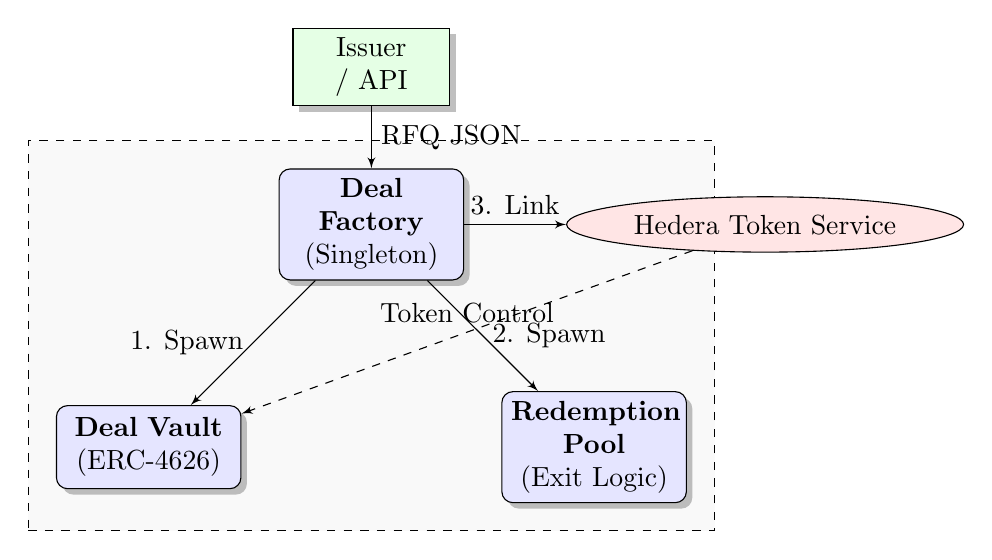
\begin{tikzpicture}[node distance = 2cm, auto]
    % Nodes
    \node [entity] (issuer) {Issuer / API};
    \node [block, below of=issuer] (factory) {\textbf{Deal Factory}\\(Singleton)};
    \node [block, below left of=factory, node distance=4cm] (vault) {\textbf{Deal Vault}\\(ERC-4626)};
    \node [block, below right of=factory, node distance=4cm] (pool) {\textbf{Redemption Pool}\\(Exit Logic)};

    % HTS
    \node [cloud, right of=factory, node distance=5cm] (hts) {Hedera Token Service};

    % Lines
    \path [line] (issuer) -- node {RFQ JSON} (factory);
    \path [line] (factory) -- node [left] {1. Spawn} (vault);
    \path [line] (factory) -- node [right] {2. Spawn} (pool);
    \path [line] (factory) -- node {3. Link} (hts);
    \path [line, dashed] (hts) -- node [above] {Token Control} (vault);

    % Background
    \begin{pgfonlayer}{background}
        \node[container, fit=(vault) (pool) (factory)] (layer) {};
    \end{pgfonlayer}
\end{tikzpicture}
\caption{Atomic Deployment of a Deal Ecosystem}
\end{figure}

% =============================================================================
% SECTION 4: DESIGN RATIONALE
% =============================================================================
\section{Design Rationale}

\subsection{Why separate the Vault from the Payment Logic?}
We utilize the \textbf{Adapter Pattern}.
\begin{itemize}
    \item \textbf{The Vault} is "dumb." It only knows how to hold Asset X and release it after Date Y. This makes it formally verifiable and chemically pure ERC-4626.
    \item \textbf{The Adapters} (Router/Pool) handle the "business." They handle the discount math ($Price = FaceValue / Yield$).
    \item \textbf{Benefit:} If we want to change from Unsecured NCDs to \textit{Secured Collateralised Lending}, we only change the Asset passed to the Vault. The Vault code remains identical.
\end{itemize}

\subsection{Why a new Vault for every Deal?}
\begin{itemize}
    \item \textbf{Asset Immutability:} ERC-4626 requires a fixed `asset()` address. Since every NCD is a new HTS Token, every NCD needs a new Vault.
    \item \textbf{Maturity Immutability:} The maturity date is hardcoded into the Vault's constructor. This provides a trustless guarantee to the investor that the date cannot be changed by an admin key.
    \item \textbf{Risk Segregation:} If Borrower A defaults on Deal A, the liquidity for Deal B is in a completely different smart contract address.
\end{itemize}

% =============================================================================
% SECTION 5: OPERATIONAL WORKFLOW
% =============================================================================
\section{Operational Run-Sheet}

\subsection{Phase 1: RFQ \& Deployment}
\begin{enumerate}
    \item \textbf{Quote:} Investor accepts 5.00\% Yield, \$1M Face Value, Dec 31 Maturity.
    \item \textbf{Mint:} Backend mints HTS Token ``NCD-DEC31''.
    \item \textbf{Spawn:} Backend calls `DealFactory.deployDeal(NCD-DEC31, USDC, Dec31)`.
    \item \textbf{Result:} A new Vault and Redemption Pool are deployed on-chain.
\end{enumerate}

\subsection{Phase 2: Investment (The Discount Entry)}
The Investor wants to buy \$1M Face Value, but only pays \$950k (Discount).

\begin{figure}[H]
\centering
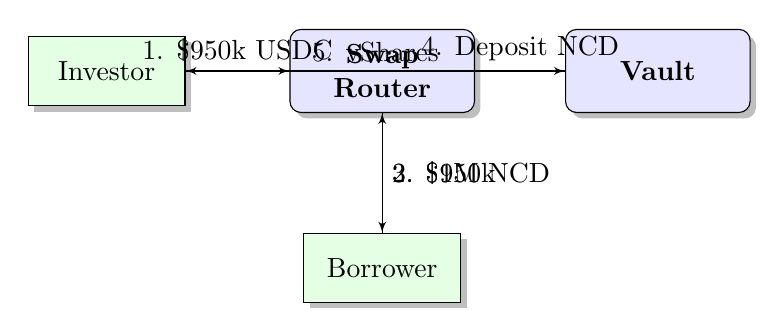
\begin{tikzpicture}[node distance = 2.5cm, auto]
    % Nodes
    \node [entity] (investor) {Investor};
    \node [block, right of=investor, node distance=3.5cm] (router) {\textbf{Swap Router}};
    \node [block, right of=router, node distance=3.5cm] (vault) {\textbf{Vault}};
    \node [entity, below of=router] (borrower) {Borrower};

    % Lines
    \path [line] (investor) -- node {1. \$950k USDC} (router);
    \path [line] (router) -- node {2. \$950k} (borrower);
    \path [line] (borrower) -- node [right] {3. \$1M NCD} (router);
    \path [line] (router) -- node {4. Deposit NCD} (vault);
    \path [line] (vault) -- node [above, bend right=45] {5. vShares} (investor);

\end{tikzpicture}
\caption{Cash Flow Diagram: The Discounted Entry}
\end{figure}

\subsection{Phase 3: Redemption (The Par Exit)}
At maturity, the Investor redeems Shares to get Face Value (in USDC).

\begin{enumerate}
    \item \textbf{Pre-Funding:} Borrower sends \$1M USDC to the \textbf{Redemption Pool}.
    \item \textbf{Action:} Investor calls `redeem` on the Pool.
    \item \textbf{Logic:}
    \begin{itemize}
        \item Pool takes vShares $\to$ Withdraws NCD from Vault.
        \item Pool burns NCD.
        \item Pool sends \$1M USDC to Investor.
    \end{itemize}
\end{enumerate}

% =============================================================================
% SECTION 6: RELATED WORK & REFERENCES
% =============================================================================
\section{Related Work \& Industry Comparison}

\subsection{Abrdn / Archax (Hedera)}
In 2022, Abrdn tokenized money market funds on Hedera.
\begin{itemize}
    \item \textbf{Architecture:} They utilize a "Permissioned Token" model. The logic is not in an open Vault but enforced via HTS Key configurations (KYC/Freeze).
    \item \textbf{Comparison:} Our proposal adds an open DeFi layer (ERC-4626) on top of the permissioned asset, allowing for greater composability with other applications while retaining HTS security.
\end{itemize}

\subsection{Ondo Finance (Ethereum)}
Ondo uses a similar "Factory" pattern for creating tranches of US Treasuries (OUSG).
\begin{itemize}
    \item \textbf{Architecture:} They separate the \textit{Fund Management} contract from the \textit{Token}.
    \item \textbf{Comparison:} Our design mirrors Ondo's separation of concerns but is optimized for the specific "Discount Security" math of the Australian market, whereas Ondo typically uses a Rebase or NAV-update model.
\end{itemize}

\section{Conclusion}

This architecture provides a robust, scalable foundation for institutional lending on Hedera. By leveraging the Factory Pattern, we ensure that every deal is chemically pure in its execution—segregated, immutable, and standard. The use of ERC-4626 ensures future compatibility with the broader DeFi ecosystem, while the Adapter pattern solves the specific complexity of settling Discount NCDs.

\end{document}
